\documentclass[conference]{IEEEtran}
\usepackage{graphicx}
\usepackage{geometry}
\usepackage{array}
\usepackage{booktabs}
\usepackage{cite}
\usepackage{amsmath,amssymb,amsfonts}
\usepackage{algorithmic}
\usepackage{graphicx}
\usepackage{textcomp}
\usepackage{xcolor}
\usepackage{tikz}
\usepackage{smartdiagram}
\usepackage{hyperref}
\usetikzlibrary{shapes, arrows, positioning}

\def\BibTeX{{\rm B\kern-.05em{\sc i\kern-.025em b}\kern-.08em
    T\kern-.1667em\lower.7ex\hbox{E}\kern-.125emX}}
\begin{document}

\title{Ultrasonic Frequency Anomaly Localization with Machine and Deep Learning\\}

\author{\IEEEauthorblockN{Evan Smith}
\IEEEauthorblockA{\textit{Ingram School of Engineering} \\
\textit{Texas State University}\\
San Marcos, USA \\
ers131@txstate.edu}
\and
\IEEEauthorblockN{Joni McCawley}
\IEEEauthorblockA{\textit{Ingram School of Engineering} \\
\textit{Texas State University}\\
San Marcos, USA \\
jwz6@txstate.edu}
\and
\IEEEauthorblockN{Antonio Grahm}
\IEEEauthorblockA{\textit{Ingram School of Engineering} \\
\textit{Texas State University}\\
San Marcos, USA \\
unw5@txstate.edu}
}
\maketitle
\begin{abstract}
TODO:
\end{abstract}
\begin{IEEEkeywords}
TODO:
\end{IEEEkeywords}
\section{Introduction \textbf{ANTONIO: TODO}}
Ultrasonic signals ($\>20 kHz$) often indicate electronic equipment malfunctions or pressurized volume integrity loss. Detecting these signals is crucial in applications where system integrity determines the habitability of an environment, such as space habitats or spaces where industrial equipment is harbored. \textbf{(DETECTING WITH MEMS $->$ LINEAR ARRAY BEAM FORMING $->$ OUR REASON FOR NOT LINEAR (HORNS) $->$ ML)} Supervised machine learning is increasingly used to monitor ultrasonic anomalies due to its ability for complex fitting, improved generalization, and continuous retraining. This project aims to use machine learning techniques to predict the location of ultrasonic anomalies using FFT data from a c array of three MEMS microphones.
\section{Background \textbf{ANTONIO: TODO}}
\textbf{validate our approach, original exec summary has good stuff.}
\section{Dataset} %why we chose it, how we collected it, what it looks like
The dataset used in this project is crucial for the development and training of our machine and deep learning models. It consists of a collection of magnitudes from ultrasonic sound signals acquired by a circular array of three MEMS microphones. The microphones are equipped with attached horns to enhance gain, but also creating a 'field of view'. When the microphones are positioned closely together, the outer two microphones are slightly angled to the right and left of the center microphone. As a result of this configuration, we will obtain five detection zones, comprising three primary regions individually created by each microphone, in addition to two secondary regions formed at the intersections of microphones 1 and 2, and 2 and 3. These regions will serve as the labels for the dataset and can be seen in Fig. \ref{fig1}.
The features of the dataset are frequency bin' magnitude components of the Fast Fourier Transform (FFT) done on the ultrasonic sound signals. Since the array consists of three channels, the microprocessor will compute the Fast Fourier Transform on each channel, resulting in three FFTs. By applying the Fast Fourier Transform (FFT) to the three channels, we extract the magnitudes of ultrasonic frequency bins present in each channel's FFT. As a result, the dataset features consist of magnitude measurements representing a signal's amplitude at various frequencies, captured by three microphone channels, each potentially containing an ultrasonic frequency anomaly. The Table \ref{tab:dataset_structure} below, is an example of how the dataset will be organized in a data frame.
\begin{figure}[htbp]
    \centering
    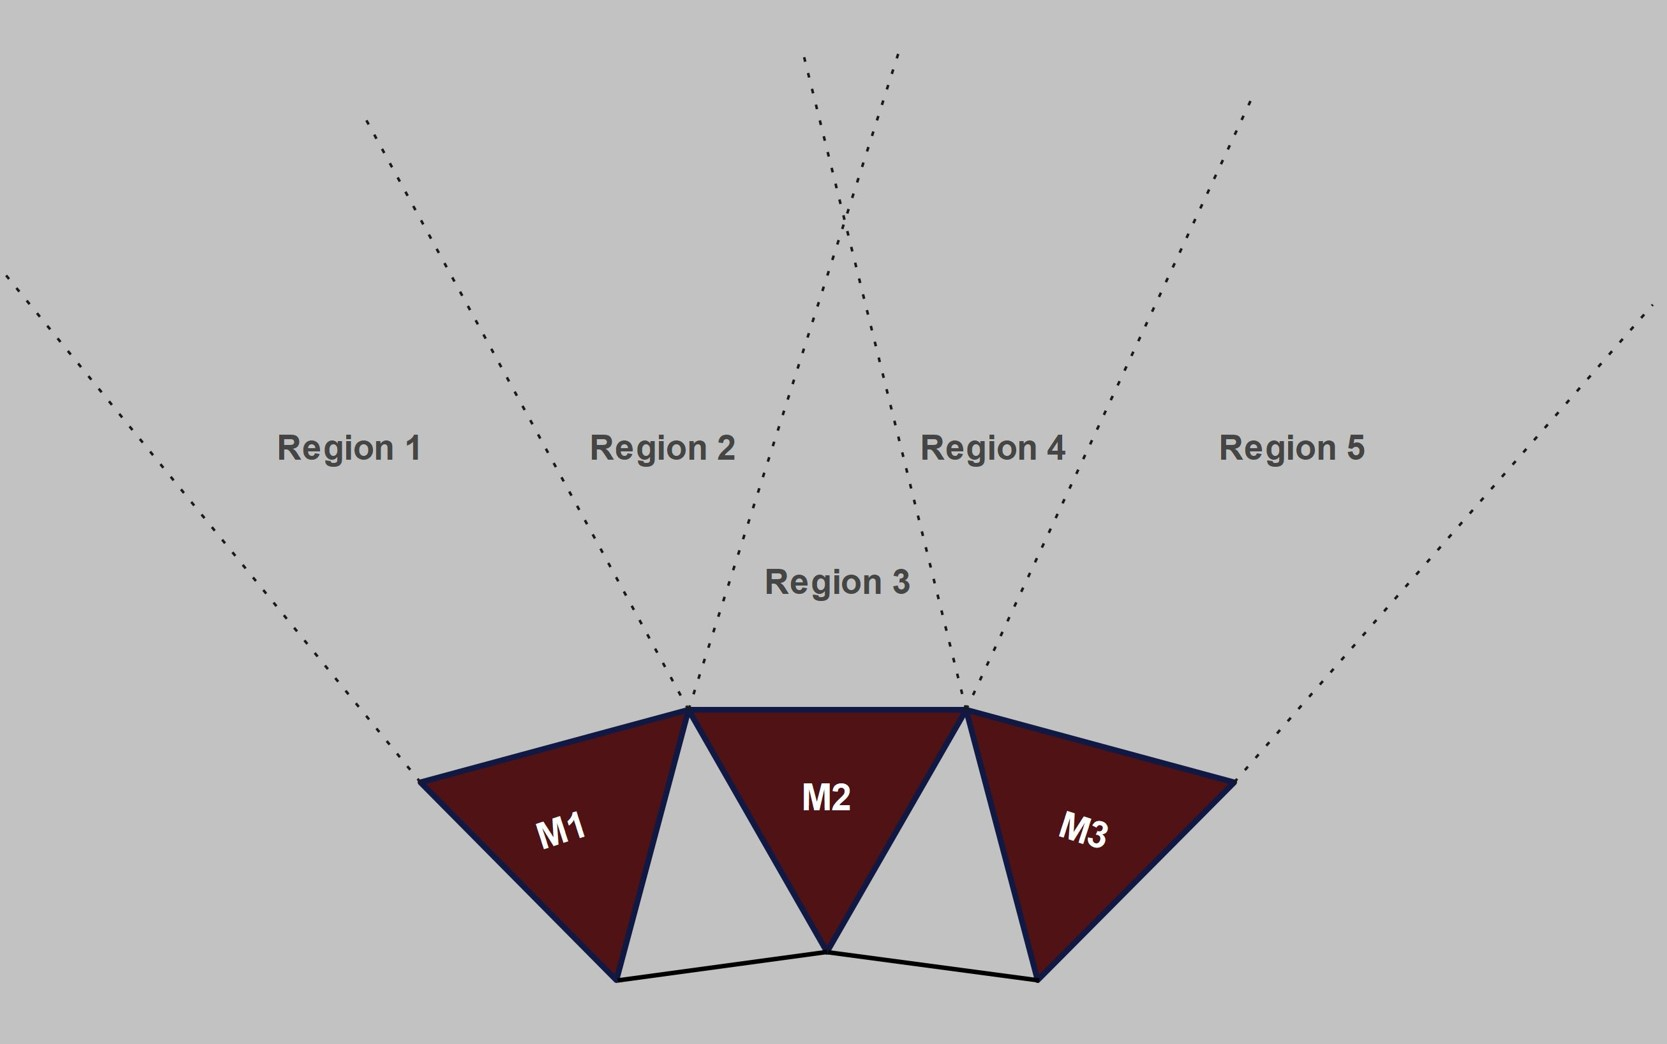
\includegraphics[width=6cm]{figs/nn/setchregions.png} % Adjust the width as needed
    \caption{Representation of MEMS microphone array and detection zones}
    \label{fig1}
\end{figure}
\subsection{Data Collection}
In the context of this machine/deep learning project, the creation of a robust and diverse dataset is a crucial step in training effective anomaly detection models. The dataset was manually generated using a custom data collection setup.
\subsubsection{Data Acquisition Setup}
The data collection process involved configuring a microcontroller to execute the anomaly detection mechanism. The microcontroller transmitted Fast Fourier Transform (FFT) data via UART to a laptop. A MATLAB live script on the laptop, configured to listen on the corresponding COM port, received and processed the transmitted data. As the microcontroller detected anomalies, it transmitted the relevant data to the MATLAB script. The script dynamically plotted the current frequency spectrum and concurrently appended the data from each anomaly detection to a CSV file named after the region from which the sample was collected.
\subsubsection{Anomaly Triggering Mechanism}
To induce anomaly detections during data collection, an ultrasonic emitter was strategically employed across various regions. The procedure involved:
\begin{enumerate}
    \item Naming the CSV file according to the region the emitter is intended to trigger.
    \item Setting the ultrasonic emitter at a specific distance from the center of the region.
    \item Maintaining this position for a specified duration to ensure equal sample distribution.
    \item After the predetermined time, repeating the process in the next region to prevent contamination of data with samples labeled in the wrong region.
\end{enumerate}
To ensure consistent regions, precise measurements of the microphones' fields of view were taken and marked on the basement floor using tape. This meticulous approach guaranteed that the regions remained identical, preventing contamination and ensuring the reliability of the dataset. Through multiple collection sessions, a total of 48,000 samples of detection data were gathered. The dataset encompasses anomalies detected at three different ranges within each region, providing a diverse and comprehensive set of examples for model training.
\begin{figure}[htbp]
    \centering
    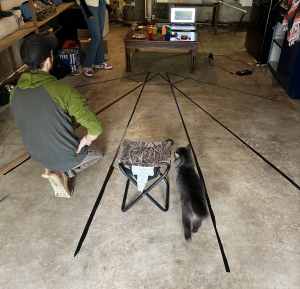
\includegraphics[width=6cm]{figs/nn/datacollectionregionslive_cropped.png} % Adjust the width as needed
    \caption{Measured fields of view created by the MEMS microphone array}
    \label{fig2}
\end{figure}
\subsection{Data Preprocessing and Analysis}
The raw dataset obtained from the anomaly detection mechanism underwent a series of preprocessing steps to prepare it for machine learning model training. Key steps in the raw data preprocessing phase included:

\begin{enumerate}
  \item \textbf{Manual Dataset Creation:} Data was manually curated by configuring a microcontroller to transmit Fast Fourier Transform (FFT) data to a MATLAB live script, which recorded anomalies in different regions.

  \item \textbf{Consistent Region Definition:} To maintain consistency, the fields of view of microphones were precisely measured and marked on the basement floor. This meticulous approach ensured uniform regions, preventing contamination.

  \item \textbf{Anomaly Triggering Process:} An ultrasonic emitter was strategically placed to trigger anomalies in different regions. This process involved careful naming of CSV files, precise emitter placement, and equal sample distribution to avoid bias.
\end{enumerate}

After the raw dataset was collected, it was preprocessed to prepare it for machine learning model training. The preprocessing steps included many of the standard techniques used in machine learning, such as standardization and dimensionality reduction. The preprocessing steps are outlined in the following sections.

\subsubsection{Standardization and Dimensionality Reduction}
To prepare the collected dataset for machine learning models, a two-step process of standardization and dimensionality reduction was employed. Standardization ensured that all features were on a consistent scale. Subsequently, dimensionality reduction techniques were applied to enhance computational efficiency and uncover underlying patterns in the data. To visualize the entire standardized dataset in a 2D plot, a UMAP and TSNE were applied to the dataset. The UMAP and TSNE plots are shown in Fig. \ref{fig3}. The plots show that the dataset isn't linearly separable, indicating that a linear model will not be able to accurately classify the data. This observation is expected since the dataset consists of magnitudes of FFTs, which are not linearly separable. The UMAP and TSNE plots also show that the dataset is not easily separable, indicating that a non-linear model will be required to accurately classify the data.
\begin{figure}[htbp]
    \centering
    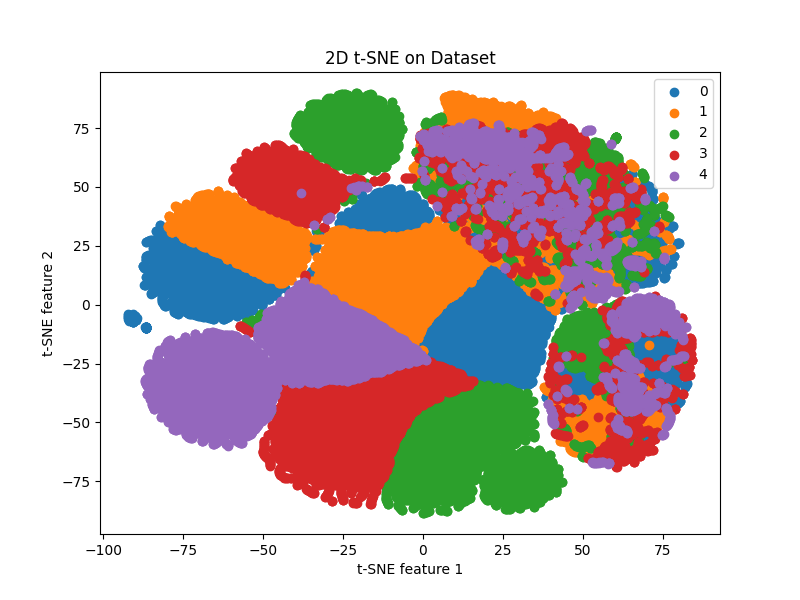
\includegraphics[width=5cm]{figs/nn/tsne.png} % Adjust the width as needed
    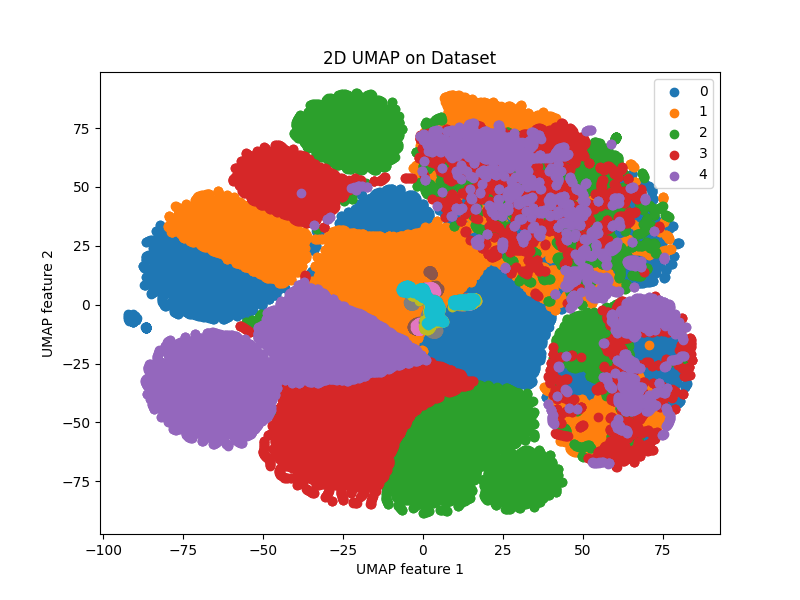
\includegraphics[width=5cm]{figs/nn/umap.png} % Adjust the width as needed
    \caption{UMAP and TSNE plots of the standardized dataset}
    \label{fig3}
\end{figure}
\subsubsection{Dimensionality Reduction Techniques}
Principal Component Analysis (PCA), Linear Discriminant Analysis (LDA) Both two-dimensional (2D) and three-dimensional (3D) projections were explored for PCA and LDA as seen in \ref{fig4} and \ref{fig5}. The 2D projections were not able to separate the data into distinct regions, indicating that a linear model will not be able to accurately classify the data. The 3D projections were able to separate the data into more distinct regions, but it isn't too clear. Thus, indicating that a non-linear model will be required to accurately classify the data. The 3D projections also show that the data is not easily separable, indicating that a non-linear model will be required to accurately classify the data.
\begin{figure}[htbp]
    \centering
    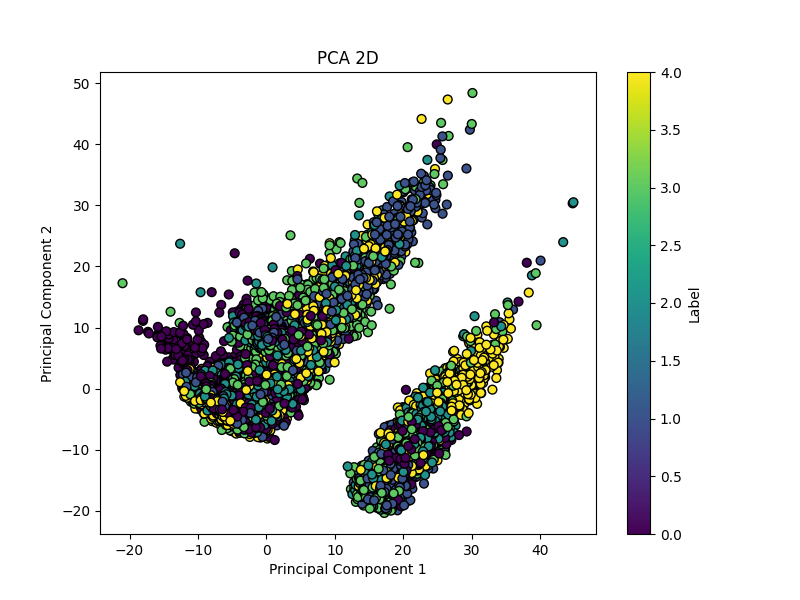
\includegraphics[width=5cm]{figs/nn/pca_2d.png} % Adjust the width as needed
    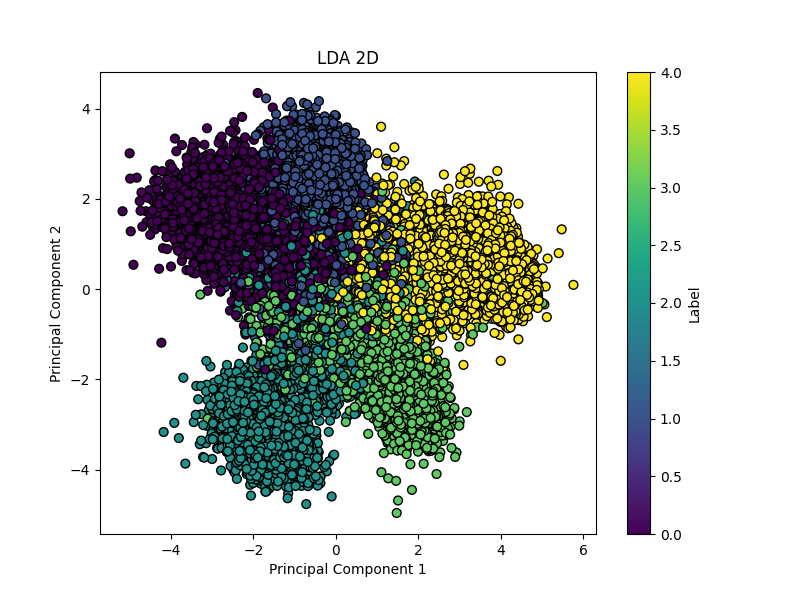
\includegraphics[width=5cm]{figs/nn/lda_2d.png} % Adjust the width as needed
    \caption{PCA and LDA 2 Component plots of the standardized dataset}
    \label{fig4}
\end{figure}

\begin{table}[bp]
    \centering
    \begin{tabular}{cccc}
        \toprule
        \textbf{Ch1\_xHz\_Mag} & \textbf{...} & \textbf{Ch3\_zHz\_Mag} & \textbf{Region} \\
        \midrule
        X dBV & ... & Z dbV & R1 \\
        X dBV & ... & Z dbV & R2 \\
        X dBV & ... & Z dbV & R3 \\
        X dBV & ... & Z dbV & R4 \\
        X dBV & ... & Z dbV & R5 \\
        \bottomrule\\
    \end{tabular}
    \caption{Structure of the Dataset}
    \label{tab:dataset_structure}
\end{table}
\section{Procedures}
Upon completion of the model training and evaluation, the system prototype operates similarly to how data is collected when an ultrasonic frequency source is detected by the microprocessor. In practical terms, the system follows these steps:
\begin{itemize}
    \item The system awaits the detection of an ultrasonic frequency.
    \item Upon detecting an ultrasonic frequency anomaly, the controller calculates the Fast Fourier Transform (FFT) on the signal containing the anomaly for each microphone channel.
    \item The resulting FFT data is then transmitted over UART to a laptop running a Python script. This script creates an instance of the selected model and loads the model weights saved during evaluation on startup. The script remains idle, waiting for a transmission over the COM port to which the MCU is connected.
    \item After receiving a transmission, the Python script preprocesses the data using the same techniques employed during training and evaluation.
    \item The processed data is then used to predict the region in which the anomaly was detected, and the corresponding region number is printed on the output console.
\end{itemize}
\begin{figure}[htbp]
    \centering
    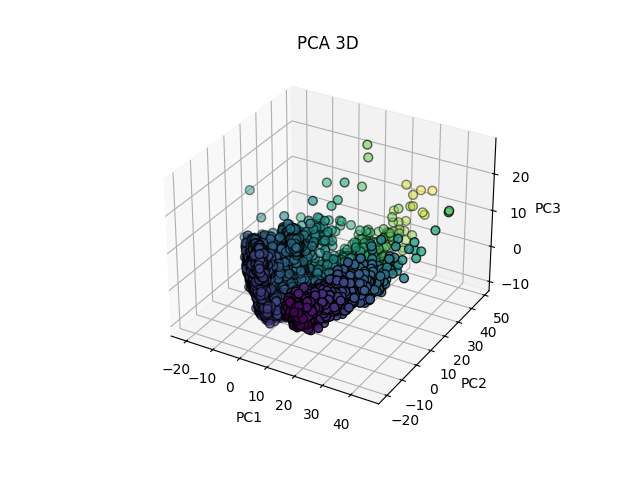
\includegraphics[width=5cm]{figs/nn/pca_3d.png} % Adjust the width as needed
    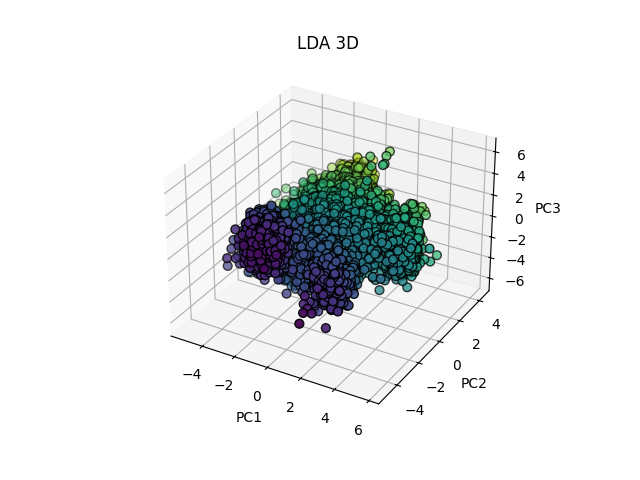
\includegraphics[width=5cm]{figs/nn/lda_3d.png} % Adjust the width as needed
    \caption{PCA and LDA 3 Component plots of the standardized dataset}
    \label{fig5}
\end{figure}
\subsubsection{Cluster Validation and Optimal Components}
To determine the optimal number of clusters, the elbow method was employed on the dataset. The analysis revealed that three clusters were optimal. This result validated the choice of three components for both LDA and PCA.
\begin{figure}[htbp]
    \centering
    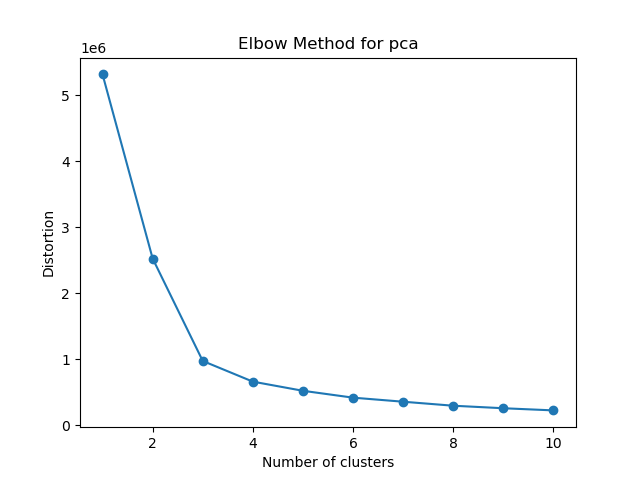
\includegraphics[width=5cm]{figs/nn/elbow.png}
    \caption{Elbow Method for Cluster Validation}
    \label{fig6}
\end{figure}
\subsection{Impact of Data Collection Strategy}
An observation during the initial data collection revealed that models trained on data collected only in the middle of regions exhibited poorer performance and showed signs of overfitting. In response, additional data was collected from short-range and long-range positions within each region. For example, when data was collected at only one distance from the center of the region, the Decision Tree model achieved training accuracy of 100\% and testing accuracy of 82.57\%. However, when data was collected at three distances from the center of the region, the Decision Tree model achieved training accuracy of 100\% and testing accuracy of 94.22\%. This observation indicates that the data collection strategy has a significant impact on the performance of the machine learning models. The additional data collected from short-range and long-range positions within each region helped the models generalize better and prevented overfitting.
The combination of standardization, dimensionality reduction, and strategic adjustment of data collection strategies resulted in a more effective dataset for training machine learning models. The optimized dataset demonstrated improved model performance, underscoring the importance of thoughtful preprocessing and analysis in enhancing the efficacy of anomaly detection models.
\section{Classification}
A collection of machine learning models and deep learning models were selected as candidates. This section will discuss the motivation behind the selection of these models and the results of their training and evaluation.
\subsection{Artificial Neural Network (ANN)}
The selection of an appropriate neural network architecture plays a pivotal role in the success of a machine learning project. In the context of our anomaly detection task with a dataset comprising 762 features, the initial neural network design was carefully crafted to address the specific characteristics and requirements of the dataset.
\subsubsection{Initial Neural Network Configuration}
The neural network was tailored to accommodate the high-dimensional nature of the dataset (762 dimensions). The input layer featured 762 neurons, ensuring comprehensive coverage of the available information.
Rectified Linear Unit (ReLU) activation functions were employed in hidden layers for their effectiveness in capturing complex relationships and preventing vanishing gradient issues.
Two hidden layers (256 and 128 neurons) facilitated hierarchical learning, enabling the model to discern intricate patterns within the high-dimensional feature space.
A Dropout layer (dropout rate: 0.2) was introduced after the first hidden layer to address overfitting concerns by promoting a more robust representation during training.
The output layer, with 5 neurons, aligned with the multi-class classification task, employing the softmax activation function for normalized probabilities across the five distinct regions.
Compilation utilized the Adam optimizer for efficiency, $'sparse\_categorical\_crossentropy'$ as the loss function for multi-class scenarios, and accuracy as the evaluation metric.
The design allowed flexibility for further optimization, enabling adjustments in the number of layers and neurons to accommodate performance and computational considerations.
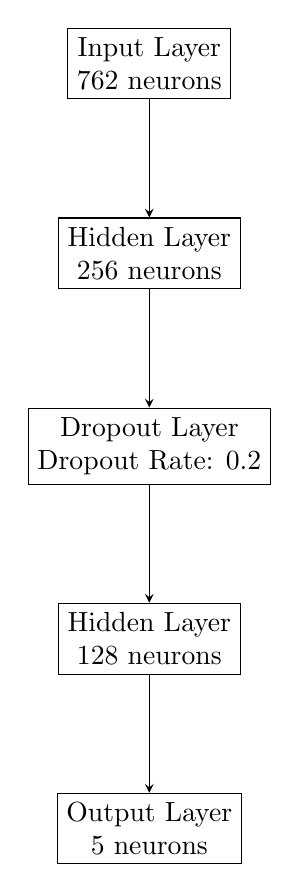
\begin{tikzpicture}[>=stealth, node distance=1.5cm]
    % Input layer
    \node[draw, rectangle, align=center] (input) {Input Layer \\ 762 neurons};
    
    % Hidden layers
    \node[draw, rectangle, align=center, below=of input] (hidden1) {Hidden Layer \\ 256 neurons};
    \node[draw, rectangle, align=center, below=of hidden1] (dropout) {Dropout Layer \\ Dropout Rate: 0.2};
    \node[draw, rectangle, align=center, below=of dropout] (hidden2) {Hidden Layer \\ 128 neurons};
    
    % Output layer
    \node[draw, rectangle, align=center, below=of hidden2] (output) {Output Layer \\ 5 neurons};

    % Arrows
    \foreach \i/\j in {input/hidden1, hidden1/dropout, dropout/hidden2, hidden2/output}
        \draw[->] (\i) -- (\j);

\end{tikzpicture}
\subsection{Model Performance Evaluation - joni}
\textbf{TODO: JONI (just add a lil bit about how we used the metrics to identify overfitting or poopoo models)}
To assess the efficiency and effectiveness of the machine learning models, various performance metrics will be employed. These metrics will help in quantifying the models' ability to predict the region in which an ultrasonic anomaly was detected. Common performance metrics include:
\begin{itemize}
   \setlength\itemsep{8pt}
   \scriptsize
   \item \textbf{Accuracy:} Accuracy measures the overall correctness of the model's predictions. It is calculated as the ratio of correct predictions to the total number of predictions.

   \item \textbf{Precision:} Precision measures the ability of the model to make correct positive predictions. It is calculated as the ratio of true positive predictions to the total positive predictions.

   \item \textbf{Recall (Sensitivity):} Recall measures the ability of the model to correctly identify positive cases. It is calculated as the ratio of true positive predictions to the total actual positive cases.

   \item \textbf{F1-Score:} The F1-Score is the harmonic mean of precision and recall. It provides a balance between these two metrics.

   \item \textbf{Confusion Matrix:} A confusion matrix will be generated to visualize the number of true positives, true negatives, false positives, and false negatives.

   \item \textbf{Receiver Operating Characteristic (ROC) Curve and Area Under the Curve (AUC):} For binary classification models, ROC curves and AUC can be used to assess model performance.
\end{itemize}
\begin{thebibliography}{00}
    \bibitem{bowler2022ultrasonic} A. L. Bowler and M. P. Pound, "A Review of Ultrasonic Sensing and Machine Learning Methods to Monitor Industrial Processes," \textit{Ultrasonics}, Elsevier, May 28, 2022. \url{https://www.sciencedirect.com/science/article/pii/S0041624X2200083X}.
\end{thebibliography}

\end{document}